\tab Ennek a modulnak a feladata a LED-fűzérek összekötése a BRAM modulokkal. Egy generikus változó által lehet definiálni, hogy hány \textbf{WS2813\_Controller} szükséges a modulban (hány LED-fűzért kell megvezérelni).
A \textbf{WS2813\_Controller} modulok automatikusan lesznek kigenerálva, a generikus változó függvényében, viszont a BRAM modulokat muszáj kézzel kigenerálni és beilleszteni az adott modulba a megfelelő helyre.

\subsubsection{Elvégzendő RT műveletek azonosítása}

\tab A modulnak a feladata már egyszerű, csak össze kell kösse a már meglévő modulokat, ezért kevés logikát is tartalmaz, kevés RT művelet azonosítható. 
A modulnak tudnia kell, hogy a \textbf{WS2813\_Controller} moduljai mikor fejezték be a küldést. Ezért szükséges ezeknek a moduloknak a \textbf{done} jelei között egy logikai ÉS művelet elvégzése.

\tab RT művelet: $done \Leftarrow Controller\_done(0) \& ... \& Controller\_done(n - 1)$


\subsubsection{Adatfüggőségek identifikálása}

\tab Mivel nagyon egyszerű RT műveletekkel meg lehet oldani az adott feladatot, nem merűlnek fel adatfüggőségek.


\subsubsection{Célregiszterek azonosítása}

\tab Nincs szükség külön célregiszterekre a feladat megoldása érdekében.


\subsubsection{Különböző fázisokban elvégzendő műveletek}
\begin{table}[H]
	\begin{center}
		\caption{WS2813\_TopLevel - Különböző fázisokban elvégzendő műveletek}
		\begin{tabular}{l|c|c|c|c}
		\textbf{Állapot} & $Controller_{reset}$     & $Controller_{start}$  & $BRAM_{enable}$ & done \\
		\hline         
        READY            & '0'                      & '0'                   & '0'             & '0'  \\
        \hline         
        INIT             & '0'                      & '0'                   & '1'             & '0'  \\
        \hline         
        RESET\_CTRLS     & '1'                      & '0'                   & $BRAM_{enable}$ & '0'  \\
        \hline         
        START\_CTRLS     & '0'                      & '1'                   & $BRAM_{enable}$ & '0'  \\
        \hline         
        SEND             & '0'                      & '0'                   & $BRAM_{enable}$ & '0'  \\
        \hline         
        FINISHED         & '0'                      & '0'                   & '0'             & '1'  \\
		\end{tabular}
	\end{center}
\end{table}

\subsubsection{Kapcsolási rajz}

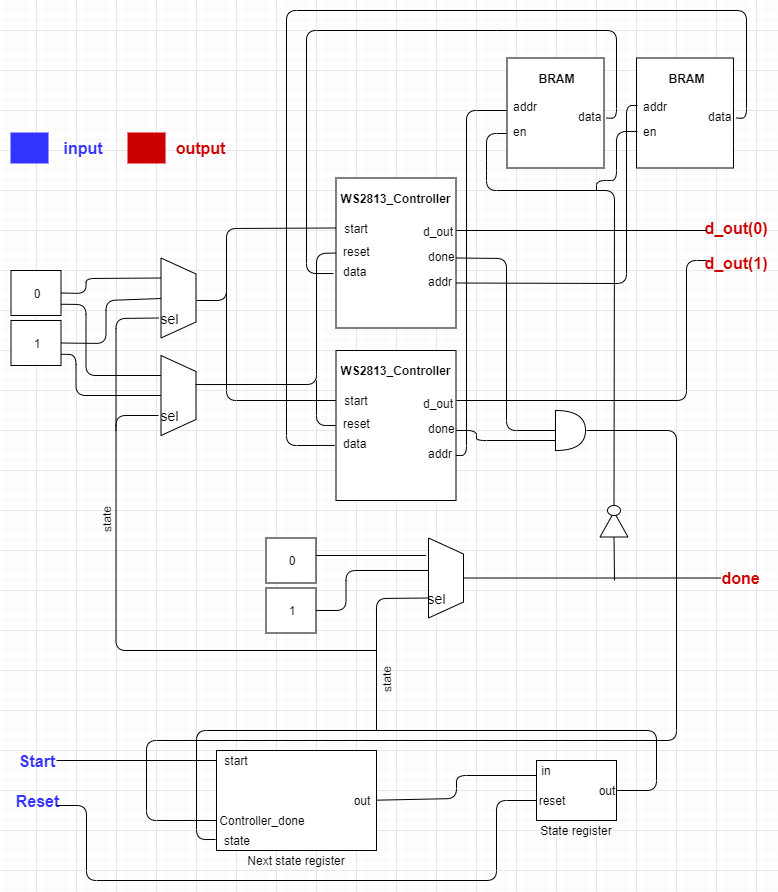
\includegraphics[scale=0.4]{WS2813_TopLevel_rtl.png}

\subsubsection{Állapotdiagram}

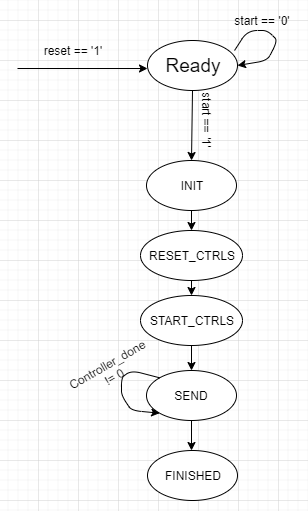
\includegraphics[scale=0.6]{WS2813_TopLevel_statedia.png}